\section{Teilaufgabe 8}
\begin{aufgabe}
    Programmieren Sie diese Steuerung mit Simulink. Wenn der Lastmoment gleich 
    null ist, ist die ideale Steuerung $S_t(s)$ das Inverse von $P_1(s)$ da 
    $S_t(s) \cdot {P_1}^{-1}(s) = 1$ (Referenzdrehzahl gleich Ist-Drehzahl). 
    Warum ist diese Steuerung nicht realisierbar? Anstatt zu ${P_1}^{-1}(s)$ 
    nehmen Sie einfach $\frac{1}{K_g}$ für $S_t(s)$ und testen Sie diese 
    Steuerung im Simulation.  Was passiert wenn der Wert von $K_g$ für die 
    Steuerung ($\frac{1}{K_g}$) nicht mehr der gleiche wie der Wert von $K_g$ 
    in der Übertragungsfunktion $P_1(s)$ ist? Was passiert wenn der Lastmoment 
    nicht null ist? Simulieren Sie diese 2 Fälle und zeigen Sie somit 2 von 
    der grossen Limitierung einer einfachen Steuerung im Vergleich zu einer 
    Regelung.
\end{aufgabe}
\[ P_1(s) = \frac{K_g}{\tau \cdot s + 1} \]
Somit ist ${P_1}^{-1}$:
\[ {P_1}^{-1}(s) = \frac{\tau}{K_g} \cdot s + \frac{1}{K_g} \]
Ein idealer Differenzierer kann nicht realisiert werden. 
\begin{figure}[h!]
    \centering
    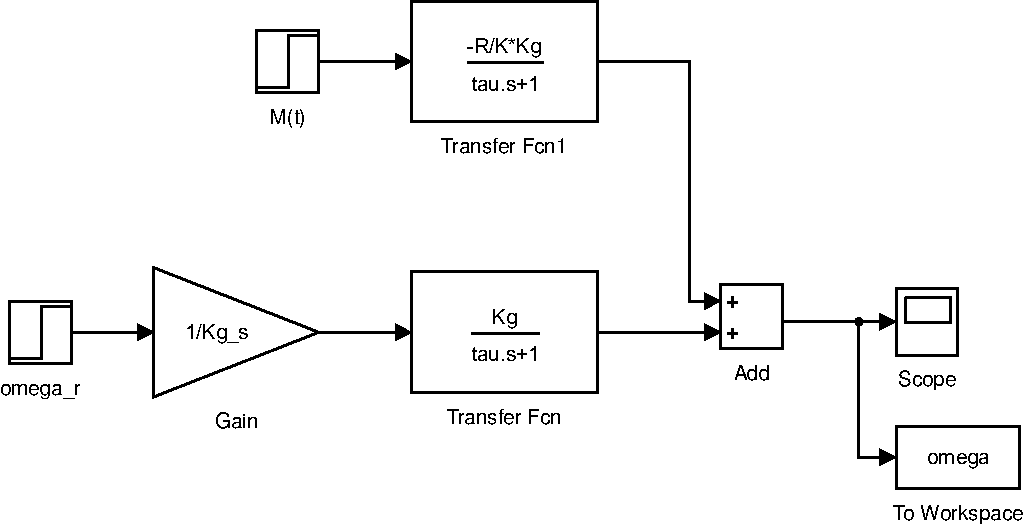
\includegraphics[width=0.6\textwidth]{08/steuerung.pdf}
    \caption{Steuerung in Simulink}
    \label{fig:03}
\end{figure}
\begin{figure}[h!]
    \centering
    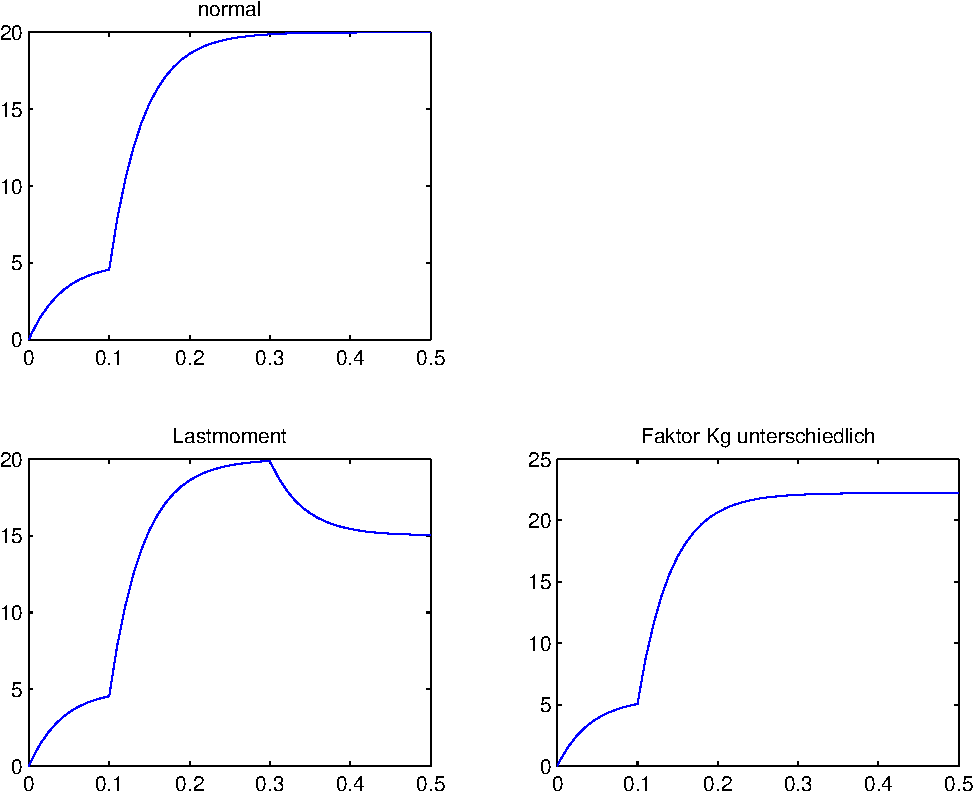
\includegraphics[width=0.6\textwidth]{08/steuerung_plot.pdf}
    \caption{Simulationsergebnis}
    \label{fig:08plot}
\end{figure}
\\
Stimmen Steuerung und Strecke nicht zusammen, ergibt sich eine Abweichung 
von der Solldrehzahl. Störungen können nicht kompensiert werden. 
